\chapter{Internship Experience}
\label{ch:internship_experience}

\section{Ops-Edge Architecture}
\label{sec:internship_experience:opsedge_architecture}

The OpsEdge Architecture, depicted in Figure~\ref{fig:opsedge_architecture}, provides a high-level overview of a cloud-based system designed to collect, process, and potentially analyze data.

\begin{figure}[h]
    \centering
    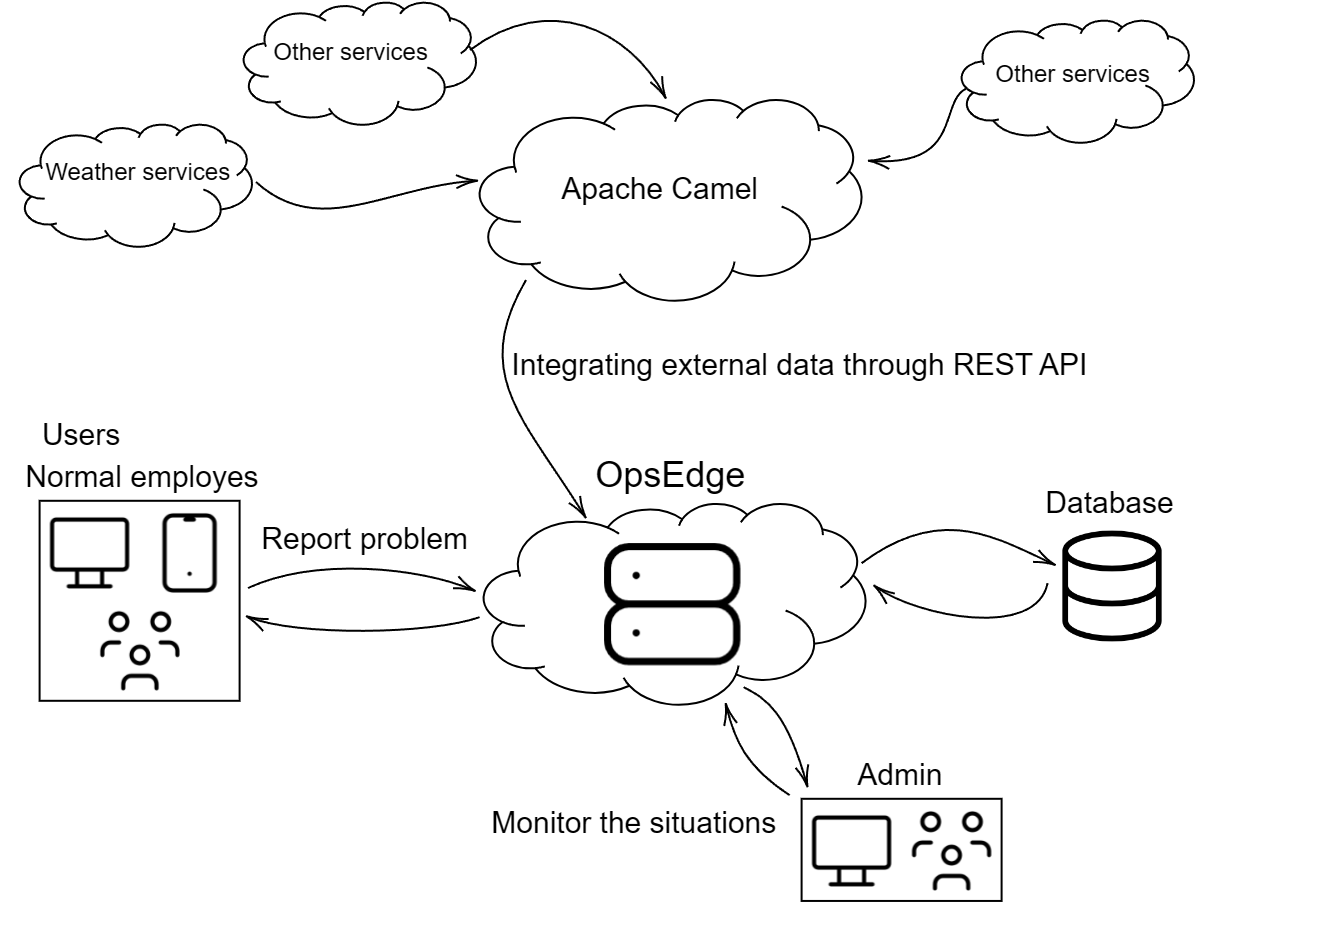
\includegraphics[width=0.9\textwidth]{gfx/opsedge-architecture.png}
    \caption{OpsEdge Architecture}
    \label{fig:opsedge_architecture}
\end{figure}

The architecture is composed of the following components:

\begin{itemize}
    \item \textbf{Users:} This layer represents the various user groups that interact with the system. It can include normal employees who report problems, and administrators who monitor situations.
    \item \textbf{OpsEdge:} This is the main component of the system. The web application is used to interact with the system, where the users can report problems, monitor the system, and analyze data.
    \item \textbf{Database:} The database stores all the data collected by the system.
    \item \textbf{Apache Camel:} This is the integration layer of the system. It is responsible for collecting data from various sources, processing it, and giving it to the OpsEdge component through a REST API\@.
    \item \textbf{Services:} These are the various services that the system can uses to integrate data with.
\end{itemize}

% TODO: Organize the content below

\section{Initializing the Project}
\label{sec:internship_experience:initializing_project}

In this section we will discuss the backend models, and how the database schema should look like. We will gonna use the Flask framework with SQLAlchemy as the ORM\@. By using an ORM, we can define the models in Python, and the ORM will take care of creating the database schema. This saves us time and effort, and allows us to focus on the business logic without having to worry about the database schema and lots of complex SQL queries.

\subsection{Managing Point of Interest with a Three-Tiered Model}
\label{subsec:internship_experience:three_tiered_model}

As the reporting system not only applicable to physical location, but also to other entities, we will refer them as Point of Interest (POI). This can be a building, a process, a condition of an item, etc. 

Effectively monitoring large number of POIs can be challenging. To address this, we go with a three-tiered model that provides an abstraction layer between different operational levels. This approach simplifies identifying troubled POIs and allows for efficient management.

\begin{itemize}
    \item \textbf{Region:} This is the highest level, representing a broad area (e.g., Building A, Building B). It serves as a high-level overview and provides context for lower levels.
    \item \textbf{Area:} This level represents a subdivision within a region (e.g., Floor 1, Floor 2, etc.). It allows for a more focused analysis compared to the region level.
    \item \textbf{POI:} This is the lowest level, representing individual locations of interest (e.g., Main lobby, Parking area, etc). It provides the most granular details about a specific location.
\end{itemize}

By having 3 levels allows us to have:

\begin{itemize}
    \item \textbf{Improved visibility:} By structuring data hierarchically, the model allows for quick identification of troubled regions and areas. This helps prioritize further investigation at the POI level.
    \item \textbf{Efficient Management:}  By focusing initial assessment at higher levels, the model reduces the need to analyze every individual POI initially. Resources can be allocated efficiently to address urgent issues.
    \item \textbf{Scalability:} The model can accommodate a large number of POIs. As the number of POIs grows, managing them remains efficient by leveraging the regional and area levels for initial screening.
\end{itemize}

\subsection{Storing the report from the users}
\label{subsec:internship_experience:storing_report}

When a user reports about a problem in their respective POIs, we need to store that information in the database. We will create a model called \textbf{Status} to store this information. To indicate how severe is the problem, we will also create a model called \textbf{Criticality}. This model will act as a reference, how critical a status is. We also need to store the user who reported the problem, so we will create a model called \textbf{User}.

\subsection{Access Control Level}
\label{subsec:internship_experience:access_control_level}

An access control is also implemented, to ensure user can only view and report the POIs that they have access to. This way, the users only need to focus on their respective areas, and not be overwhelmed by the whole system.

\subsection{Group}
\label{subsec:internship_experience:group}

As the system grows, managing users can be challenging. Especially when admins need to manage access control of each users with their respective POIS\@. To facilitate easier management of users, A group feature will be added. This feature will allow administrators to group various POIS with similar characteristics, such as location, type, etc. Additionally, this feature will allow administrators to assign users to specific groups, streamlining user management and access control.

\subsection{Audit}
\label{subsec:internship_experience:audit}

An audit trail is implemented to capture all changes occurring at the database level. This comprehensive approach empowers both administrators and data analysts to conduct further analysis of system activity.

This provide us with several benefits:

\begin{itemize}
    \item \textbf{Improved Situational Awareness:} By providing a record of specific changes and the users responsible, the audit trail facilitates the identification of potential issues. This ultimately leads to faster response times and informed decision-making by administrators.
    \item \textbf{Granular Data Analysis:} The rich dataset of user activity and data modifications captured by the audit trail allows for in-depth analysis of trends, user behavior, and potential areas for improvement by data analysts.
    \item \textbf{Improved Data Integrity:} The audit trail serves as a historical record, enabling verification of past actions and ensuring the continued accuracy and reliability of data.
\end{itemize}

Therefore, another model called \textbf{AuditLog} will be created to store this information, and an event listeners from SQLAlchemy will be used to automatically log the changes.

\subsection{Communication}
\label{subsec:internship_experience:communication}

To facilitate easier communication between users, we will implement a real-time group chat in Area level. This feature will allow users to discuss issues, share information, and collaborate more effectively. This provides a centralized platform for communication, reducing the need for multiple tools and ensuring that all relevant parties are kept informed. A Notification feature will also be implemented to allow Administators to send important messages to all or specific users. There are also Comments feature that allows users to comment on a specific report. This feature will help users to provide additional information, ask questions, or provide feedback on a particular issue.

\subsection{Real-time data and notifications}
\label{subsec:internship_experience:realtime_data_notifications}

To improve the data visualization in dashboard, real-time data are required, such as current open statuses, critical statuses, etc. To achieve this, Socket.IO are used to send the data to the frontend in real-time without having to refresh the page. By utilizing the audit log, we can also send notifications to the users when a specific event occurs, such as a new report, a status change, etc.

\subsection{User interface}

The backend models are now defined, and the database schema is created. Now we need to create a user interface to interact with the system. It will be created using React as the frontend library, and Mantine as the UI framework. The user interface should have at least the following functionalities:

\begin{itemize}
    \item \textbf{Login:} Users should be able to login to the system.
    \item \textbf{POIs:} Users should be able to view list of POIS and their respective status.
    \item \textbf{Report:} Users should be able to report a problem in their respective POIs.
    \item \textbf{Dashboard:} Admins should be able to view a dashboard that summarize important informations, such as open reports, critical reports, etc.
\end{itemize}

\section{Integration with External Services}
\label{sec:internship_experience:integration_external_services}

Now that the functionalities within the system are implemented, we are ready to combine the app with external services. This will allow us to enrich the data and provide more value to the users. In this case, we are going to integrate the weather data from `Deutsche Wetterdienst' (DWD) to provide real-time weather information. we will create a POI called `Frankfurt Weather' in the app. Then, using message oriented middleware Apache Camel, we retrieve the data from DWD using their REST API\@, process it, and then forward the data through a REST API to the OpsEdge component. To make it easier to update a status for a POI, we use `shortname' attribute in the POI model and create an endpoint for this, so that we do not have to use the ID of the poi everytime we want to update its status from external.

TODO: INSERT PICTURE